\documentclass{article}
\usepackage[T1]{fontenc}
\usepackage{lmodern}
\usepackage{graphicx}
\usepackage{amsmath,amssymb}
\usepackage[a4paper,margin=2cm]{geometry}
\usepackage[absolute,overlay]{textpos}
\setlength{\TPHorizModule}{1mm}
\setlength{\TPVertModule}{1mm}
\usepackage[indonesian]{babel}
\usepackage{hyperref}
\setlength{\emergencystretch}{2em}
% unit: Halaman 29

\begin{document}

% === Halaman 29 (llm) ===

\begin{itemize}
  \item Di dalam sistem operasi Unix, \texttt{ROT13} adalah fungsi menggunakan \textit{Caesar cipher} dengan pergeseran $k = 13$
\end{itemize}

\vspace{60mm}

Sumber gambar: Wikipedia

% deskripsi: Diagram ilustrasi cara kerja ROT13 yang menunjukkan pemetaan huruf alfabet A-M ke N-Z dan contoh enkripsi kata 'HELLO' menjadi 'URYYB'.
% bbox normalisasi: [0.1300, 0.2400, 0.6600, 0.8100]
\begin{textblock*}{111.30mm}(27.30mm,71.28mm)
\noindent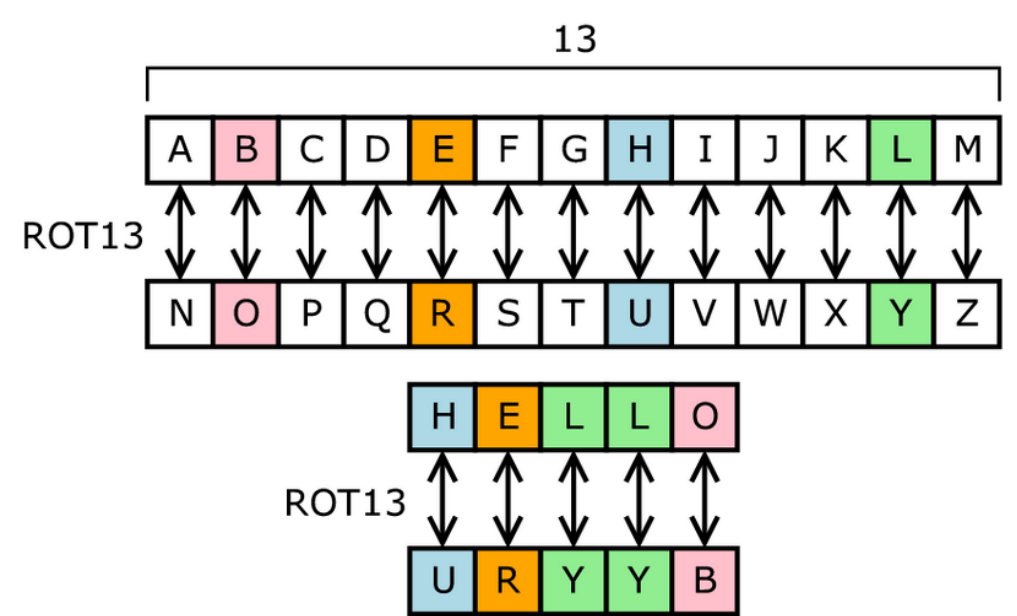
\includegraphics[width=111.30mm,height=169.29mm]{../../images/llm/page_029_img_01.png}%
\end{textblock*}

\end{document}
